\section{Overview}
For the aims to be met, it is important that we have a strong idea about what will be needed to be done in order to meet the objectives set. In this section, we will be discussing the core algorithms, core data-structures and also the user-interface of the library. The library will now be referred to as the NeuralDot library. 

\subsection{Algorithms}
The main algorithms that will be used in the making of the NeuralDot library is as follows:
\begin{enumerate}
    \item Neural Networks
    \item Optimisation
    \item Matrix Operations
\end{enumerate}

I will be discussing each of these algorithms in detail separately along with their respective pseudo-codes
\subsubsection{Neural Networks}
There are many variations of neural networks each with its own purpose, however the main type of neural networks I will be focusing on will be feed-forward neural networks and convolutional neural networks. Feed-forward NNs are the most basic type of NNs and also the backbone for many other variations there are. 
\\ \\
Throughout this paper, we will be using the standard notation to avoid any unnecessary confusion
\\
\begin{itemize}
\centering
\item[] 
$n_x$ : Input size \\
$n_y$ : Output size \\
$L$ : Number of layers in Neural Network \\
$n^{[l]}_h$ : Number of hidden units in layer $l$ \\
$m$ : Number of examples in data set \\
$X \in \mathbb{R}^{n_x \times m}$ : Input matrix, can also be referred to as $a^{[0]}$ \\
$x^{(i)} \in \mathbb{R}^{n_x}$ : $i^{th}$ example represented as a column vector \\
$Y \in \mathbb{R}^{n_y \times m}$ : Label matrix for $X$ \\
$y^{(i)} \in \mathbb{R}^{n_y}$ : Output label for the $i^{th}$ example \\
$W^{l} \in \mathbb{R}^{n_h^{l-1} \times n_h^{l}}$ : Weight matrix in layer $l$ \\
$b^{[l]} \in \mathbb{R}^{n^{[l]}_h}$ : Bias vector in layer $l$ \\
$z^{[l]} \in \mathbb{R}^{n^{[l]}_h}$ : Product vector in layer $l$ \\
$g^{[l]}$ : Activation function in layer $l$ \\
$a^{[l]} \in \mathbb{R}^{n^{[l]}_h}$ : Activation vector in layer $l$ \\
$\hat{y} \in \mathbb{R}^{n_y}$ : Predicted output vector. Can also be denoted as $a^{[L]}$
\end{itemize}

Here is an example of a simple Neural Network, with the notation included

\begin{figure}[H]
    \centering
    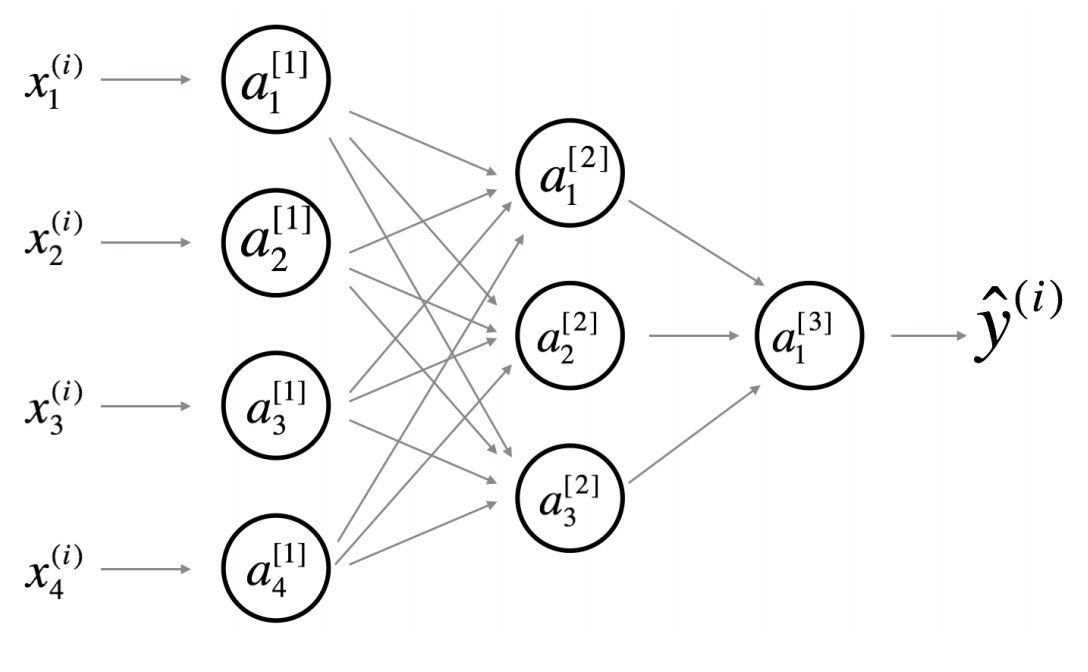
\includegraphics[width=7cm]{Design/Overview/Algorithms/NeuralNetworks/NeuralNetworkDiagram.png}
    \caption{Neural Network Example}
    \label{fig:my_label}
\end{figure}
This network is called a 2 layer network, as it has 1 hidden layer and one output layer.
\subsubsubsection{Forward Propagation} \label{SForwardProp}
Forward Propagation, also referred to as inference, is used to make a prediction given a set of inputs. The inference process for a specific layer in a neural network works as follows:
\begin{enumerate}
    \item The inputs are multiplied by the corresponding weights for that layer and then finally a bias is added, which results with the corresponding $z^{[l]}$ for that layer.
    \item Once the $z^{[l]}$ has been calculated for that layer, the activation's are then calculated using the corresponding $g^{[l]}$ for that layer, which results in $a^{[l]}$.
\end{enumerate}
This process is then repeated throughout every layer until the final layer where the error is calculated.
Using the notation we have established, we can now write this mathematically as: 
\\
\begin{center}
$a^{[l]} = g^{[l]}(z^{[l]})$ \\ 
where $z^{[l]} = W^{[l]}a^{[l-1]} + b^{[l]}$ 
\end{center}

In pseudo-code this may be written as:

\begin{algorithm}[H]
\caption{Dense Forward Propagation Algorithm}\label{DenseForewardProp}
\begin{algorithmic}[1]
\State $net \gets$ Network being used to make prediction
\State $x \gets$ mini-batch
\\
\For{\texttt{each $layer$ in $net$}}
\State $x = Matrix.matmul(layer.w, x) + layer.b$
\State $x = layer.act(x)$
\EndFor
\Return $x$
\end{algorithmic}
\end{algorithm}

Forward propagation for the convolutional layers is the same to that of the dense layers, the only difference being is that instead of matrix multiplication being the operator, the operator is now cross-correlation with both the 3d volumes. In pseudo-code this can be now written as:

\begin{algorithm}[H]
\caption{Convolution Forward Propagation Algorithm}\label{ConvForewardProp}
\begin{algorithmic}[1]
\State $net \gets$ Network being used to make prediction
\State $x \gets$ mini-batch
\State $stridesx \gets$ User Defined
\State $stridesy \gets$ User Defined
\State $padding \gets$ User Defined
\\
\For{\texttt{each $layer$ in $net$}}
\State $x = Volume.conv2d(layer.filter, x, stridesx, stridesy, padding) + layer.b$ (Applying 2d convolution, using x as input and filter as the kernel, with strides = (stridesx, stridesy) )
\State $x = layer.act(x)$
\EndFor 
\Return $x$
\end{algorithmic}
\end{algorithm}
\subsubsubsection{Back-propagation} \label{SBack-propagation}
Back-propagation, is another algorithm with many variations which will be discussed further in the section \ref{Optimisers}. Although there are many techniques for back-propagation they all have the same goal; reduce the error of the network. Therefore the essence of back propagation is to find the correct weight matrix that approximates a given function to an appropriate degree of accuracy in a given interval. Back-propagation, is a \textbf{recursive} algorithm that uses \textbf{memoization} to back-propagates throughout the network to find the \textbf{derivative} of each weight w.r.t (with respect to) a cost. The cost being used, will be set before training and is different for each task.
The notation that will be used in explaining back-propagation will be:

\begin{center}
    $E$ : denotes the error/cost function begin used \\
    $\alpha$ : denotes the learning rate used for back-prop \\
    $\delta^{l}$ : denotes the derivative of the bias matrix $b^{l}$ with respect to the cost function i.e $ \delta^{l} = \frac{\partial E}{\partial b^{l}}$ \\
    $\cdot$ : denotes the hadamard product
\end{center}

The equations, that will be used for back-propagation for a \textbf{Dense} layer will be:
\begin{center}
    $\delta^{l} = ((W^{[l+1]})^{T}\delta^{[l+1]}) \cdot g'^{[l]}(z^{[l-1]})$ \\
    $\frac{\partial E}{\partial W^{l}} = \delta^{l}(a^{[l-1]})^T$ \\
    $\frac{\partial E}{\partial b^{l}} = \delta^{l}$
\end{center}

In summation form this may be written as:

\begin{center}
    $\delta^{l} = \sum_{m} \delta_{m}^{l+1}w_{m,k}$ \\
\end{center}

%write that it took entire night to2 test the network
% explain what cdot represents

The equations, that will be used for back-propagation for a \textbf{Conv} layer will be:
\begin{center}
    $\delta^{l} = \delta^{l+1}_{x,y} \cdot rot_{180^\circ}(w^{l+1}_{x,y}) f'(a^{l}_{x,y})$ \\
    $\frac{\partial E}{\partial W^{l}_{x,y}} = \delta^{l}_{x,y} \cdot f(rot_{180^\circ} (o^{l-1}_{x,y}))$ \\
    $\frac{\partial E}{\partial b^{l}} = \delta^{l}$
\end{center}
In these equations, $w$ denotes a Volume, i.e a lists of matrices with equal dimensions.

In summation form the gradient of the error w.r.t $w^{l}$, in a conv net will be:

\begin{equation*}
    \delta^{l} = rot_{180^\circ} \{\sum_{m=0}^{k_{1} -1} \sum_{n=0}^{k_{2}-1} \delta_{i+m,j+n}^{l+1} w_{m,n}^{l+1}f'(x_{i,j}) \}
\end{equation*}

Finally, the corresponding updates for a layer in the net will be:

\begin{center}
    $W := W - \alpha \frac{\partial E}{\partial W}$ \\
    $b := b - \alpha \frac{\partial E}{\partial b}$
\end{center}
These updates will be applied to every layer in the network on each iteration.

These equations, can be easily derived by extending the chain-rule to matrix multiplication, i.e by using the lemma $\frac{\partial x^Ta}{\partial x} = a$

In pseudo-code this may be written as:
\begin{algorithm}[H]
\caption{Back-propagation Algorithm - Dense Layer}\label{StandardBackpropagation}
\begin{algorithmic}[1]
\State $net \gets$ Network being trained
\State $x \gets$ mini-batch
\State $y \gets$ labels for mini-batch
\\
\State $\hat{y} = forewardPop(x)$
\State $error = \hat{y} - y$
\State $db = [error \times net.gradact(net.last)]$ ($db$ is a list containing the gradient w.r.t the biases for each layer)
\State $dw = [net.layer(-2) \times db.last()]$ (net.layer is a list containing the gradient w.r.t the weight matrices of each layer)
\\
\For{\texttt{each $layer$ in $net$ step -1}}
\State $db.add(matrix.matmul(layer.w.T, deta.last) \cdot net.gradact(layer))$ (Adding the gradient of the loss w.r.t $b^{[layer]}$)
\State $dw.add(layer.act, db.last)$ (Adding the gradient of loss w.r.t  $W^{[layer]}$)
\EndFor
\Return $dw, db$  in the network
\end{algorithmic}
\end{algorithm}

These back-propagation algorithms require a sample of the training data. If each image is used for one back propagation, this is known as stochastic gradient decent, whereas if every image is used in the training sample, then this is known as batch-gradient descent. Batch-gradient descent is more prone to local minimas, however it can take less time to train the network, whereas stochastic gradient descent can take more time but is less prone to locals minimas. Therefore, it is important that the user selects something in between by splitting the training data into different batches each. This is known as mini-batch gradient descent. Therefore, stochastic gradient descent and batch-gradient descent are just special cases for mini-batch gradient descent when $m_b = 1$ and $m_b = m$ where $m_b$ is the mini-batch size, respectively.
\subsubsubsection{Loss-Functions}
The back-propagation algorithms in section \ref{SBack-propagation} relied on a loss function. The loss function, also referred to as the cost function, measures how bad the network is performing. Therefore, the goal of the network is to minimise the loss function, which is done through the use of the back-prop algorithm. This allows the network to learn from the data by minimising the cost function, thus a decreasing loss function implies that the net is learning from the data and a converging loss function implies that the learning is slowing down possibly due to the net having learnt the data, or reaching a global/local minimum. There are a wide array of cost function that are available, however the two most commonly used are: \textbf{soft-max} and 
\textbf{squared error}. 

Minimising a function, is a classic problem in calculus and relies upon the derivative of the function. Furthermore, the back-propagation algorithm in section \ref{SBack-propagation} relies upon the derivative of the loss function. Therefore, it is necessary to be able to compute the derivative of the cost function as it is used to back-propagate throughout the network.

\subsubsubsubsection{Squared-error}
The squared-error loss function measures the average of the sum of the squared error for each data-point.

In mathematical form, the squared-error and its derivative may be written as: 

\begin{center}
    $ E = \frac{1}{2m} \sum^m{(\hat{y}-y)^2}$ \\
    $ \frac{dE}{d\hat{y}} = \hat{y} - y $
\end{center}


These results can be proved by using the chain-rule, i.e using the result $\frac{dy}{dt} = \frac{dy}{dx} \frac{dx}{dt}$

The squared error cost function is commonly used for regression tasks, image-recognition and also used to train many other type of ML models besides neural networks.

\subsubsubsubsection{Soft-max cost function}
The soft-max function, unlike the squared error is most commonly used for multiclass classification. Multiclass classification unlike binary classification, where the data has to belong in one of 2 sets, enables the model to classify objects into more than 2 groups. This is useful for recognition system, where the model is looking out for many different objects at the same time.

Unlike the squared error, softmax works very differently compared to the squared error. The softmax loss function is usually composed of a loss function and an activation function, which is the actual softmax activation function. The loss function being used is usually the cross-entropy loss function.

The softmax activation function works by exponentiating each element in the input vector and then dividing by the sum of this vector. This results in a vector that represents the probability that a given element at an index represent the probability of the image belonging to that class.

Using mathematical notation, the softmax activation function and its respective derivative may then be written as:

\begin{center}
    $ \hat{y} = \frac{e^{z_c}}{\sum_c^{n_y} {e^{z_c}}}$\\
    where $z$ is the product vector and $z_c$ represents the $c_{th}$ item in that vector. An important point to note that since this is the last layer, the length of this vector will be $n_y$ \\
    $ \frac{dE}{d\hat{y}} = \hat{y} * (1-\hat{y}) $
\end{center}

Finally, the cross-entropy loss function works by taking in the vector of probabilities($\hat{y}$) of each class and then applying the natural logarithm to the reciprocal of each element in this vector. Each element is then multiplied by its corresponding $y_i$ which produces a vector, whose elements are then summed up which produces the output of the cross-entropy loss function. 

Using mathematical notation, the cross-entropy activation function and its respective derivative may then be written as:

\begin{center}
    $ E = \sum_c^{n_y} -y_{c}{ log(\hat{y}_{c})} $ \\
    $ \frac{dE}{d\hat{y}} = \hat{y} - y $ \\
    An interesting point to note is that the derivative for the squared error and the cross-entropy loss function is the same.
\end{center}


\subsubsection{Optimisers} \label{Optimisers}
As discussed in the previous section, we have seen that by using matrix calculus we can formulate an algorithm to back-propagate through the neural network to find the respective derivatives for each weight matrix. Once these derivatives have been found, the most basic way to update the weights is as shown in the section \ref{SBack-propagation}. However, there are many other alternatives which have shown to work much better. The alternative optimisation methods that I will also be implementing are:
\begin{itemize}
    \item Momentum Optimisation
    \item RMS Optimiser
    \item Adaptive Moment Estimation (ADAM) Optimiser
\end{itemize}

\subsubsubsection{Momentum Optimiser} \label{SMOM}
Momentum is an improvement on the traditional method of back-propagation. The traditional method of back-propagation is very susceptible to the problem of local minima. This means that $\frac{\partial E}{\partial W} = 0$ and the network stops learning, even though the error function could still be reduced further. 

Momentum, is an alternative approach that uses an extra parameter called the "momentum" term that is used to calculate the variable "velocity" on each update. The intuition behind this is that when the gradient is high, i.e the network is learning, the velocity parameter also increases, and when the learning is slow the velocity parameter also reduces. This effect allows the network to be less susceptible to local minimas. The pseudo algorithm for Momentum is as shown in Algorithm \ref{Momentum}

\begin{algorithm}[H]
\caption{Momentum}\label{Momentum}
\begin{algorithmic}[1]
\State $\alpha \gets$ User defined, default 0.01
\State $\beta \gets$ User defined, default 0.9
\State $T \gets$ User defined Number of iterations

\State $t \gets 0$ (Initialise time step)
\State $v_{dw} \gets 0$ Setting the Momentum term for $W$
\State $v_dw \gets 0$ Setting the Momentum term for $b$
\\
\For{\texttt{$t<T$}}
\For{\texttt{each $layer$ in $net$}}
\State compute $\frac{\partial E}{\partial w}, \frac{\partial E}{\partial b}$ using back-prop with mini-batch
\\
\State $dw = \frac{\partial E}{\partial w}$
\State $db = \frac{\partial E}{\partial b}$
\\
\State $v_{dw} = \beta v_{dw}  + (1-\beta)dw$ (calculating the new momentum term for w)
\State $v_{db} = \beta v_{db}  + (1-\beta)db$ (calculating the new momentum term for b)
\\
\State $W = W-\alpha v_{dw}$ (Updating weights using the weight momentum term)
\State $b = b-\alpha v_{db}$ (Updating bias using the bias momentum term)
\EndFor
\EndFor
\end{algorithmic}
\end{algorithm}
\subsubsubsection{RMS Optimiser} \label{SRMS}
RMS optimiser, is very similar to the momentum optimiser. One key difference between momentum and RMS prop however, is that RMS is not very susceptible to quick gradient changes. This is much better, as very quick gradient changes can lead to the network overshooting the local minimum and thus diverging. RMS achieves this by keeping a running average of the magnitude of the gradients and dividing the next gradient by this average so that the gradient values are approximately normalised. This can lead to much better results and has shown to out-beet momentum in many cases. The pseudo-code for the RMS optimiser is as shown in Algorithm \ref{RMSOptimizer}

\begin{algorithm}[H]
\caption{RMS Optimiser}\label{RMSOptimizer}
\begin{algorithmic}[1]
\State $\alpha \gets$ User defined, default 0.01
\State $\beta \gets$ User defined, default 0.9
\State $t \gets 0$ (Initialise time step)
\State $T \gets$ User defined Number of iterations 
\State $s_{dw} \gets 0$ RMS term for the weights
\State $s_{db} \gets 0$ RMS term for the biases
\\
\For{\texttt{$t<T$}}
\For{\texttt{each $layer$ in $net$}}
\State compute $\frac{\partial E}{\partial w}, \frac{\partial E}{\partial b}$ using back-prop with mini-batch
\\
\State $dw = \frac{\partial E}{\partial w}$
\State $db = \frac{\partial E}{\partial b}$
\\
\State $s_{dw} = \beta s_{dw}  + (1-\beta)dw^2$
\State $s_{db} = \beta s_{db}  + (1-\beta)db^2$
\\
\State $W = W-\alpha \frac{dw}{\sqrt{s_{sw}} + \epsilon}$ (Updating the weights using the normalised gradient values)
\State $b = b-\alpha \frac{db}{\sqrt{s_{sb}} + \epsilon}$ (Updating the biases using the normalised gradient values)
\EndFor
\EndFor
\end{algorithmic}
\end{algorithm}
\subsubsubsection{Adaptive Moment Estimation (Adam) Optimiser} \label{SADAM}
Adaptive Moment Estimation, or Adam for short, is another approach regularly used to minimise the cost function. Currently, Adam is one of the most used optimises used mainly due to its high-performance in computer vision problems. Therefore, I will also be implementing the Adam optimisation algorithm. The respective pseudo-code for the Adam algorithm is as shown in Algorithm \ref{AdamOptimizer}. 

\begin{algorithm}[H]
\caption{Adam Optimiser}\label{AdamOptimizer}
\begin{algorithmic}[1]
\State $\alpha \gets$ User defined, default 0.01
\State $\beta_1 , \beta_2 \in [0,1)$ Exponential decay rates for moment estimates
\State $m_{dw} \gets 0$ (Initialise $1^{st}$ moment vector for weight matrix)
\State $v_{dw} \gets 0$ (Initialise $2^{nd}$ moment vector)
\State $m_{db} \gets 0$ (Initialise $1^{st}$ moment vector for bias matrix)
\State $v_{db} \gets 0$ (Initialise $2^{nd}$ moment vector)
\State $t \gets 0$ (Initialise time step)
\State $T \gets$ User defined Number of iterations 
\\
\For{\texttt{$t<T$}}
\For{\texttt{each $layer$ in $net$}}
\State compute $\frac{\partial E}{\partial w}, \frac{\partial E}{\partial b}$ using back-prop with mini-batch
\\
\State $dw = \frac{\partial E}{\partial w}$
\State $db = \frac{\partial E}{\partial b}$
\\
\State $m_{dw} = \beta_1 m_{dw}  + (1-\beta_1)dw$
\State $v_{dw} = \beta_2 v_{dw} + (1-\beta_2)dw^2$
\\
\State $m_{db} = \beta_1 m_{db}  + (1-\beta_1)db$
\State $v_{db} = \beta_2 v_{db} + (1-\beta_2)db^2$
\\
\State $\hat{m_{dw}} = \frac{m_{dw}}{1-\beta_1^t}$
\State $\hat{m_{db}} = \frac{m_{db}}{1-\beta_1^t}$
\\
\State $\hat{v_{dw}} = \frac{v_{dw}}{1-\beta_2^t}$
\State $\hat{v_{db}} = \frac{v_{db}}{1-\beta_2^t}$
\\
\State $W = W-\alpha \frac{\hat{m_{dw}}}{\sqrt{\hat{v_{dw}}} + \epsilon}$
\State $b = b-\alpha \frac{\hat{m_{db}}}{\sqrt{\hat{v_{db}}} + \epsilon}$
\EndFor
\EndFor
\end{algorithmic}
\end{algorithm}

\subsubsection{Matrix Operations}
Neural Networks would be impossible without the help of matrices to vectorise their implementation. Therefore, it is crucial for my project to use matrices for the computationally expensive tasks. Some key algorithms, I will be using are:
\begin{itemize}
    \item Matrix Multiplication
    \item Convolution
    \item Matrix Transpose
    \item Basic Matrix Operations
\end{itemize}

\subsubsubsection{Matrix Multiplication} \label{SMatrixMultiplication}
Matrix multiplication will be used to propagate throughout a neural network. Being $O(n^3)$, it is crucial that we implement it efficiently, otherwise it would mean that the neural network runs incredibly slow when the number of neurons used increase exponentially. The pseudo-code for Matrix Multiplication is as shown in Algorithm \ref{MatrixMultiplication}. 

\begin{algorithm}[H]
\caption{Matrix Multiplication}\label{MatrixMultiplication}
\begin{algorithmic}[1]
\State $A \gets $User defined Parameter
\State $B \gets $User Defined Parameter
\\
\State $n = A.shape(0)$
\State $m = B.shape(1)$
\\
\State $C \gets $ Matrix(n, m) '$C$ will be the resulting matrix of matrix multiplication
\For{\texttt{$1 \leq i \leq n$}} (Looping over the columns of A)
\For{\texttt{$1 \leq j \leq m$}} (Looping over the rows of B)
\State $C_{ij}$ = 0
\For{\texttt{$1 \leq k \leq n$}} (Iterating over rows \& columns of A and B, respectively and summing the products)
\State $C_{ij} = C_{ij} + (A_{ik}*B_{jk})$
\EndFor
\EndFor
\EndFor
\Return C
\end{algorithmic}
\end{algorithm}
In mathematical terms this can be neatly written as:
\begin{align}
    c_{ij} = \sum_{k=1}^{m} a_{ik}b_{kj}
\end{align}

\subsubsubsection{Convolution} \label{SConvolution}
Convolution is another operation that is widely used in deep-learning. Convolution, or more correctly known as cross-correlation, is used in image recognition as it allows the network to learn a representation that is equivalent to translations. This speeds up learning, as a traditional deep-net would require many training iterations for it to learn this kind of inter-relationship of a given image. The pseudo-code for convolution is as shown in Algorithm \ref{Convolution}
\begin{algorithm}[H]
\caption{Convolution}\label{Convolution}
\begin{algorithmic}[1]
\State $M \gets $User defined Matrix - Input for the convolution operation
\State $kernel \gets $User Defined Matrix
\State $stridesx \gets$User Defined integer
\State $stridesy \gets$User Defined integer
\\
\State $h_{kernel} \gets kernel.shape(0)$ (kernel.shape(0) returns the height of the kernel)
\State $w_{kernel} \gets kernel.shape(1)$ (kernel.shape(1) returns the width of the kernel)
\State $h_m \gets M.shape(0)$
\State $w_m \gets M.shape(0)$
\\
\State $c \gets $ Matrix($\frac{h_{kernel} - h_{m}}{stridesy} + 1$, $\frac{w_{kernel} - w_{m}}{stridesx} + 1$) ($c$ will be the output matrix for the convolution operation)
\\ \\
(The Following code will now use a striding window to stride over the input $M$ using the kernel)
\For{\texttt{$0 \leq i \leq h_m$ step $stridesy$}}
\For{\texttt{$0 \leq j \leq w_m$ step $stridesx$}}
\State $c_{ij} = dotsum(kernel, m.item[i, i+h_{kernel}, j, j+w_{kernel}])$ (dotsum is a function that multiplies each matrices element-wise and then sums up the element of the matrix)
\EndFor
\EndFor
\Return C
\end{algorithmic}
\end{algorithm}

In convolutional networks, the input can also have a depth, meaning the convolution operation is applied on a volume instead of a matrix. The dotsum in this case is the same, but this time the kernel is also multiplied by each layer in the input to produce a volume, whose elements are then summed up. Furthermore, the kernel being used can also be a volume. The process is again very similar, with the only difference being that the convolution operation uses each layer of the kernel and convolves it with the input. This generates a volume as the output of the convolution operation.

In mathematical terms, a convolution operation can be written as follows:
\begin{align}
    (f*g)[n] = \sum_{-\infty}^{\infty} f^{*}(m)g[m+n]
\end{align}
\subsubsubsection{Matrix Transpose}
The transpose of a matrix is used to back-propagate throughout a neural network. It is used many times, therefore an efficient algorithm is required. Therefore, I have decided that instead of transposing an actual matrix, instead keep track of the state of the matrix using a variable called $tState$. This means when indexing the $ij_th$ item from a matrix return the $ij_th$ item if $tState$ is set to $"False"$, otherwise return the $ji_th$ item. This provides an efficient method of transposing a matrix, as traditional algorithms require transposing a matrix every time the transposed matrix is required, which is an $O(n^2)$ operations. Therefore, by using this approach we can solve this problem in $O(1)$ time.

The corresponding pseudo-code will be:
\begin{algorithm}[H]
\caption{Indexing Matrix}\label{IndexingMatrix}
\begin{algorithmic}[1]
\State $m \gets$ User-defined Matrix being used to index item
\State $i \gets $ User defined integer (Used to select the $i^{th}$ row)
\State $j \gets $ User defined integer (Used to select the $j^{th}$ column)
\\
\If{$tState = False$}
\State \Return $m(i,j)$
\Else
\State \Return $m(j,i)$    
\EndIf
\end{algorithmic}
\end{algorithm}

Therefore, the Pseudo-code for transposing a matrix will be:
\begin{algorithm}[H]
\caption{Transposing Matrix}\label{TransposingMatrix}
\begin{algorithmic}[1]
\State $tState = \bar{tState}$ (Inverting the tState boolean variable)
\end{algorithmic}
\end{algorithm}
\subsubsubsection{Basic Matrix Operations}
Some basic matrix operations that I will be using is as follows:
\begin{itemize}
    \item Addition and subtraction of 2 matrices
    \item Element wise Multiplication
    \item DotSum of 2 matrices
    \item Applying a function $f(x)$ element-wise to a matrix
    \item Applying an arbitrary function $f(x_1, x_2)$ between 2 matrices
    \item Reshaping a matrix - including reshaping a matrix to a volume
    \item Cloning a given matrix
    \item Adding columns and rows to a matrix
    \item Joining two matrices
    \item Max-pooling a matrix
    \item Rotating the items of a matrix
    \item Normalising matrices
\end{itemize}

The pseudo-code for the reshaping of a matrix is as follows:

\begin{algorithm}[H]
\caption{Reshaping Matrix}\label{Backpropagation}
\begin{algorithmic}[1]
\State $M \gets$ Matrix being reshaped
\State $rows \gets$ number of rows in resulting matrix
\State $cols \gets$ number of columns in the resulting
\State $i \gets$ Indexing of matrix
\\
\If{$matrix.shape(0)\times matrix.shape(1) \neq rows \times cols$}
\State Throw exception("Matrix dimensions do not conform for reshaping") (Exception was thrown here, as the number of elements in both matrices should be the same for reshaping to take place)
\EndIf
\State $C \gets$ matrix(rows, cols)
\For{\texttt{each $d$ in M}} (Iterating over each element in the matrix $M$)
\State $C_{ trunc(i/cols),{(i\mod cols)}+1} = d$ (Setting the values of matrix $C$ by placing each element row-wise)
\State $i+=1$
\EndFor
\Return $C$
\end{algorithmic}
\end{algorithm}

\begin{algorithm}[H]
\caption{2 to 1 function applied element-wise on 2 matrices}\label{2 to 1 function}
\begin{algorithmic}[1]
\State $X \gets$ Matrix the function will be applied on
\State $Y \gets$ Matrix the function will be applied on
\\
\State $f(x,y) \gets$ function that will be applied to both matrices
\State $C \gets$ Matrix that will be returned
\State $i=0$
\If{$X.shape <> Y.shape$}
\State Throw exception("Matrix dimensions do not conform") (Exception was thrown here as both matrices must have same dimensions for this function to be applied)
\EndIf
\For{\texttt{each $d_{x}, d_{y}$ in X,Y}} (looping over each element in matrix $X$ and $Y$)
\State $C_{ trunc(i/cols),{(i\mod cols)}+1} = f(d_{x}, d_{y})$ (Output of the function is assigned to the matrix $C$, which is being filled row-wise)
\State $i+=1$
\EndFor
\\
\Return $C$
\end{algorithmic}
\end{algorithm}

\begin{algorithm}[H]
\caption{1 to 1 function applied element-wise on matrix}\label{1 to 1 function}
\begin{algorithmic}[1]
\State $X \gets$ Matrix that function will be applied
\\
\State $f(x) \gets$ function that will be applied to both matrices
\State $C \gets$ Matrix that will be returned
\State $i=0$
\For{\texttt{each $d_{x}$ in X}} (looping over each element in matrix $X$)
\State $C_{ trunc(i/cols),{(i\mod cols)}+1} = f(d_{x})$ (Output of the function is assigned to the matrix $C$, which is being filled row-wise)
\State $i+=1$
\EndFor
\\
\Return $C$
\end{algorithmic}
\end{algorithm}

One crucial aspect of machine learning is data processing. This is extremely important as the data needs to be processed properly for the ML models to work well. Therefore, I will be adding as much functionality as I can to allow the user to process their data as much as possible. This will include functions such as remove cols/rows, rotating matrices, inversing the oneHot operation on a matrix, padding a matrix and many other functions to make the manipulation of data easy for the user. These functions will come extremely handy when the user is dealing with images as data for conv-nets, which will require volumes, and many times the data is in RGB format, which is essentially a volume of depth 3. Therefore, if the user would wanted to manipulate and process their data to make the training of the net as easy as possible, it is important that all the most used functions are all predefined, as the most important aspect of my library is to make machine learning as easy as possible. Therefore, I will be one step closer to achieving this goal, as the user will not need to define these functions which could be a daunting tasks especially for beginners thus putting off many people before even getting their hands on the machine learning stuff. Furthermore, from the pseudo-code, for the back-propagation and forward propagation algorithms, it is clear that I will be using many of these matrix operations.
\section{Data-Structures \& Diagrams}
\begin{figure}[H]
    \centering
    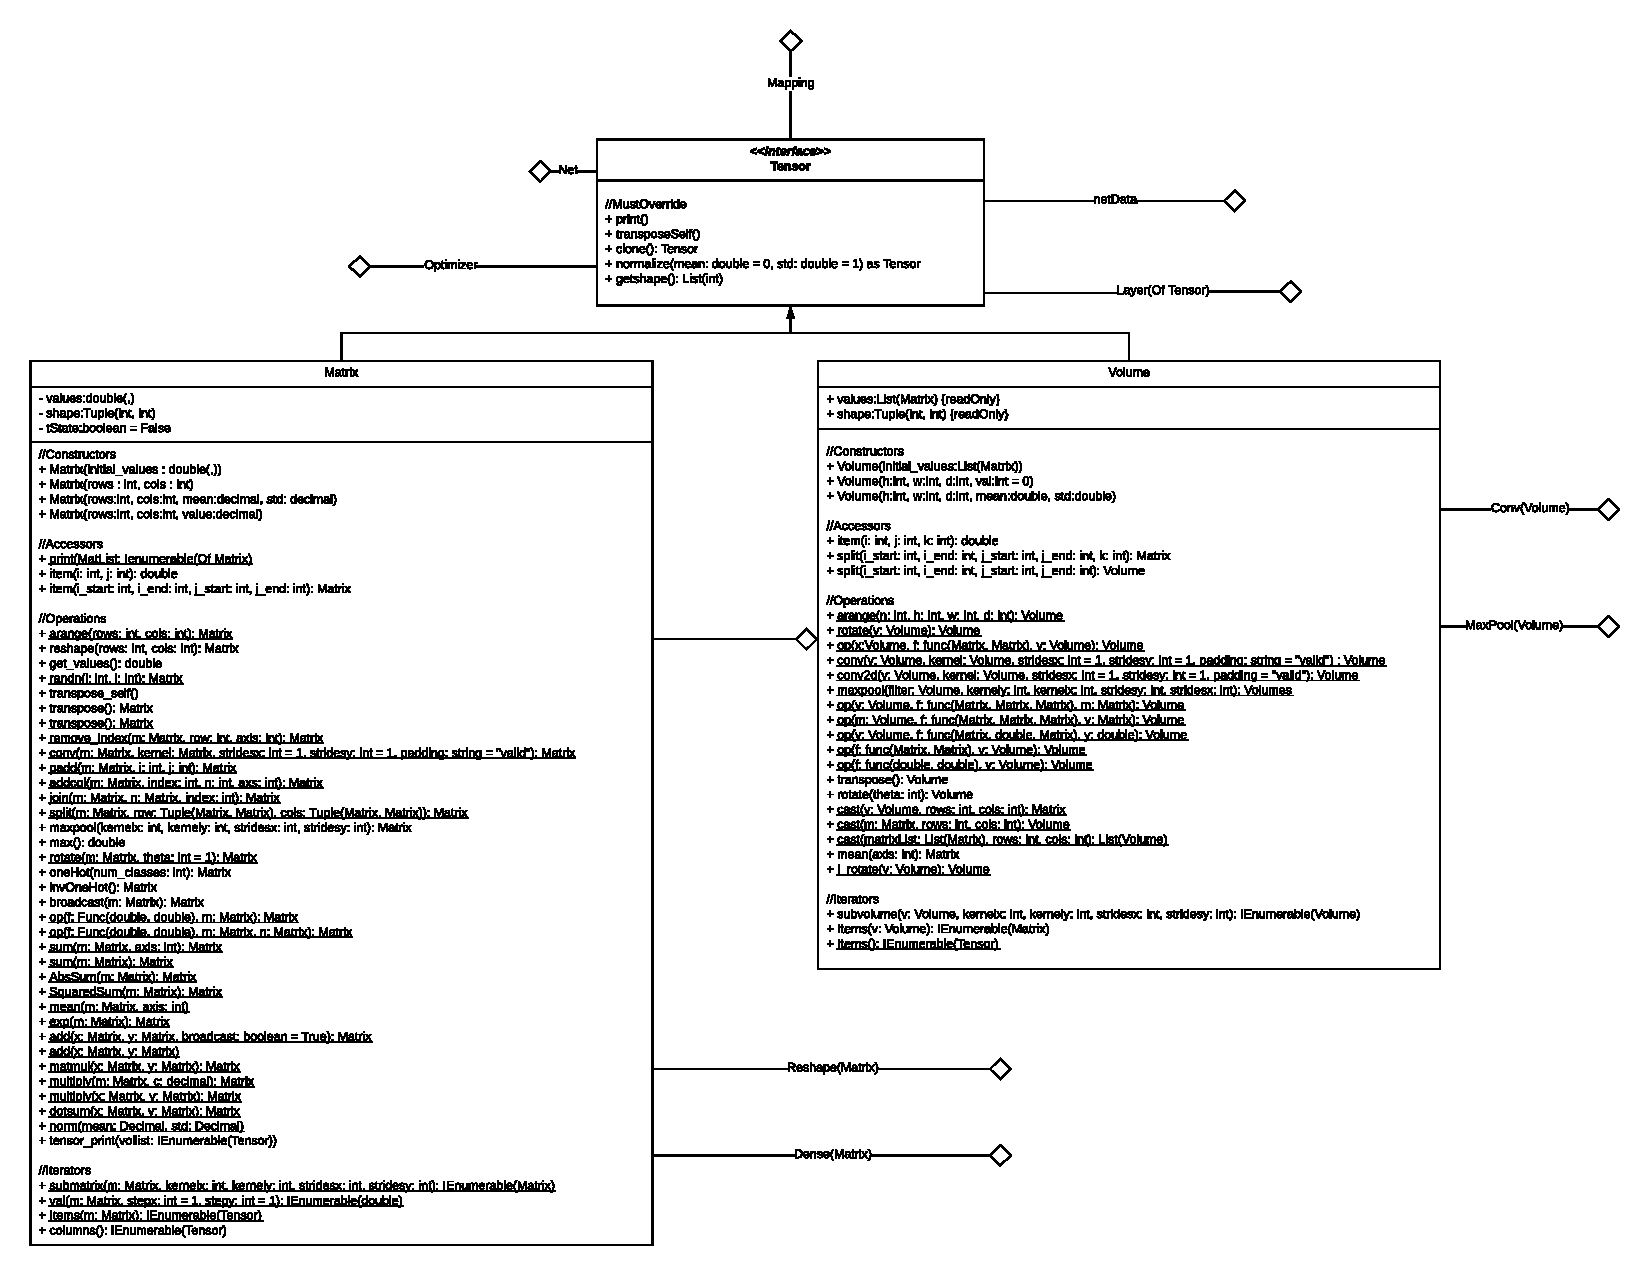
\includegraphics[width=18cm, height=18cm, angle=90]{Design/Overview/UMLCharts/NeuralDotUMLSeperated-Tensor.pdf}
    \caption{Class Diagram for NeuralDot Library - Tensors}
    \label{fig:Class Diagram for NeuralDot Library - Tensors}
\end{figure}

\begin{figure}[H]
    \centering
    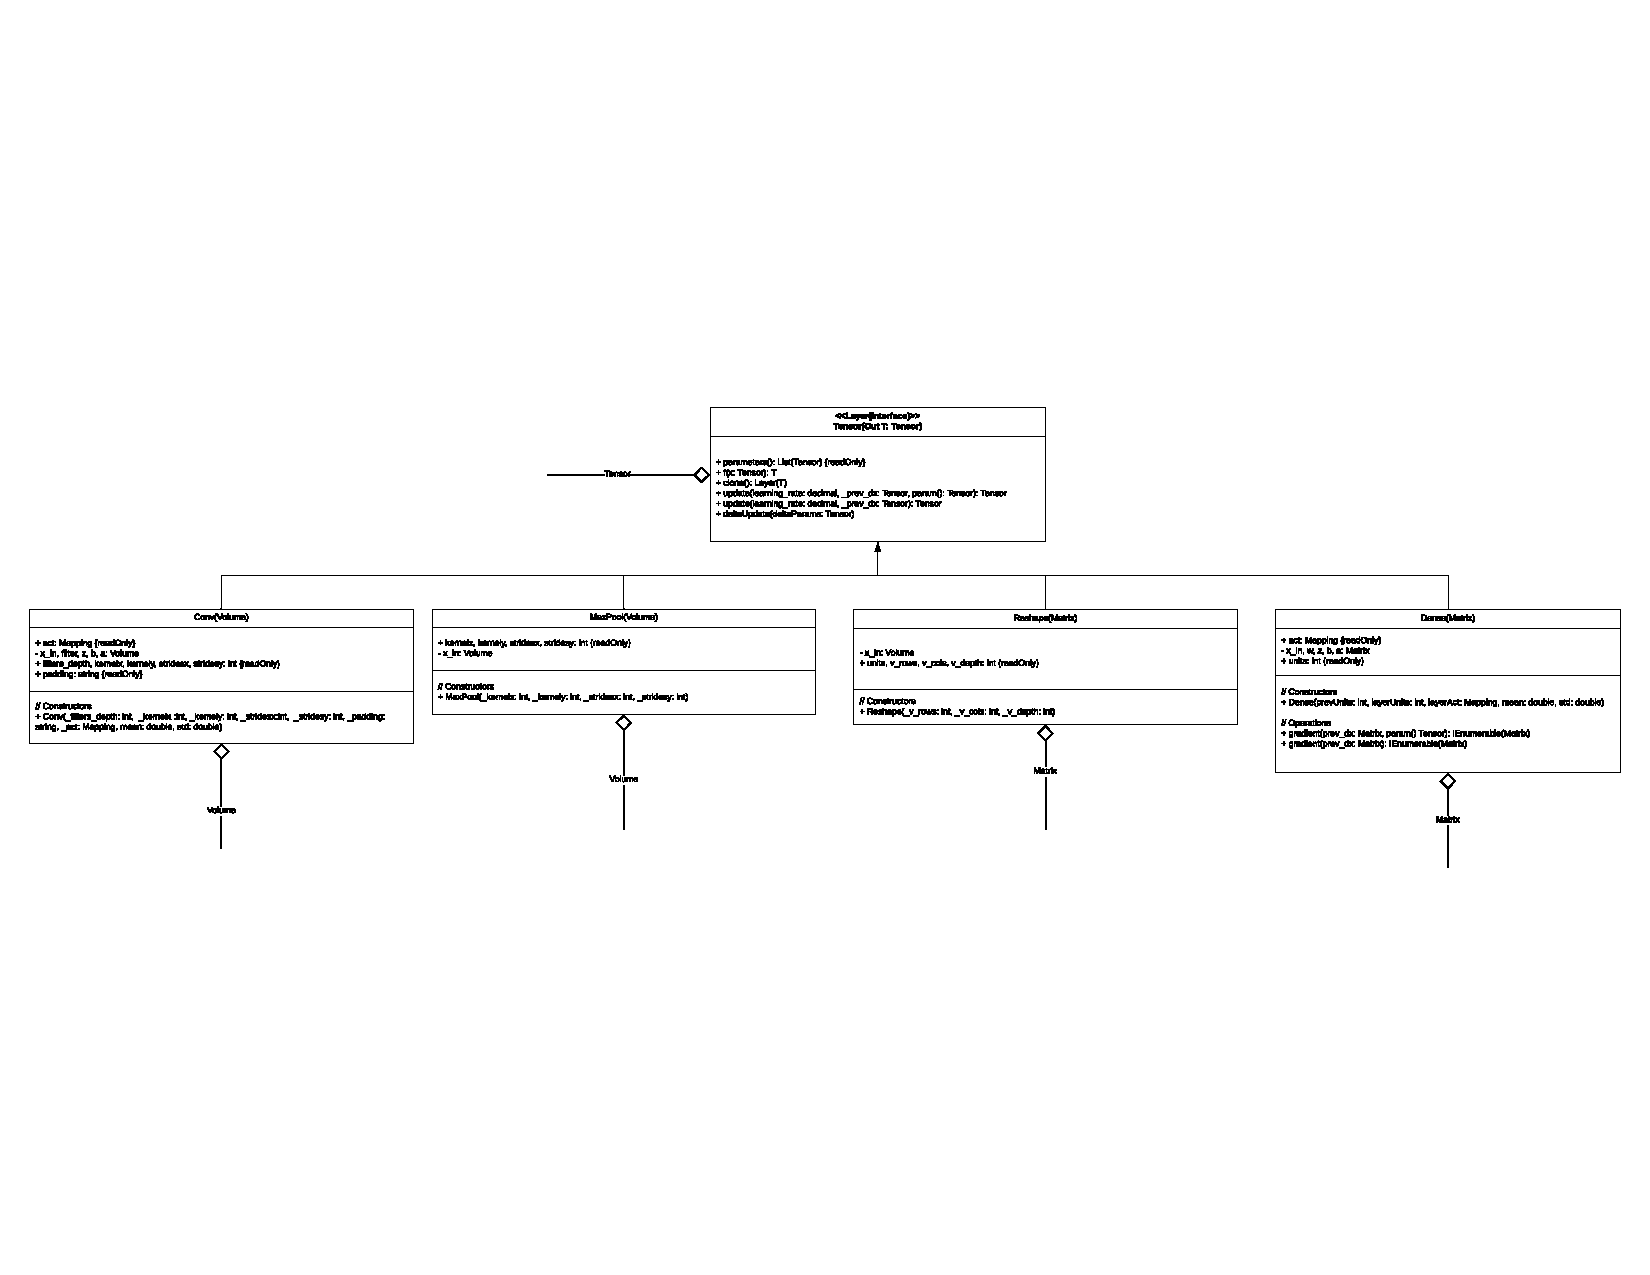
\includegraphics[width=18cm, height=18cm, angle=90]{Design/Overview/UMLCharts/NeuralDotUMLSeperated-Layer.pdf}
    \caption{Class Diagram for NeuralDot Library - Layers}
    \label{fig:Class Diagram for NeuralDot Library - Layers}
\end{figure}

\begin{figure}[H]
    \centering
    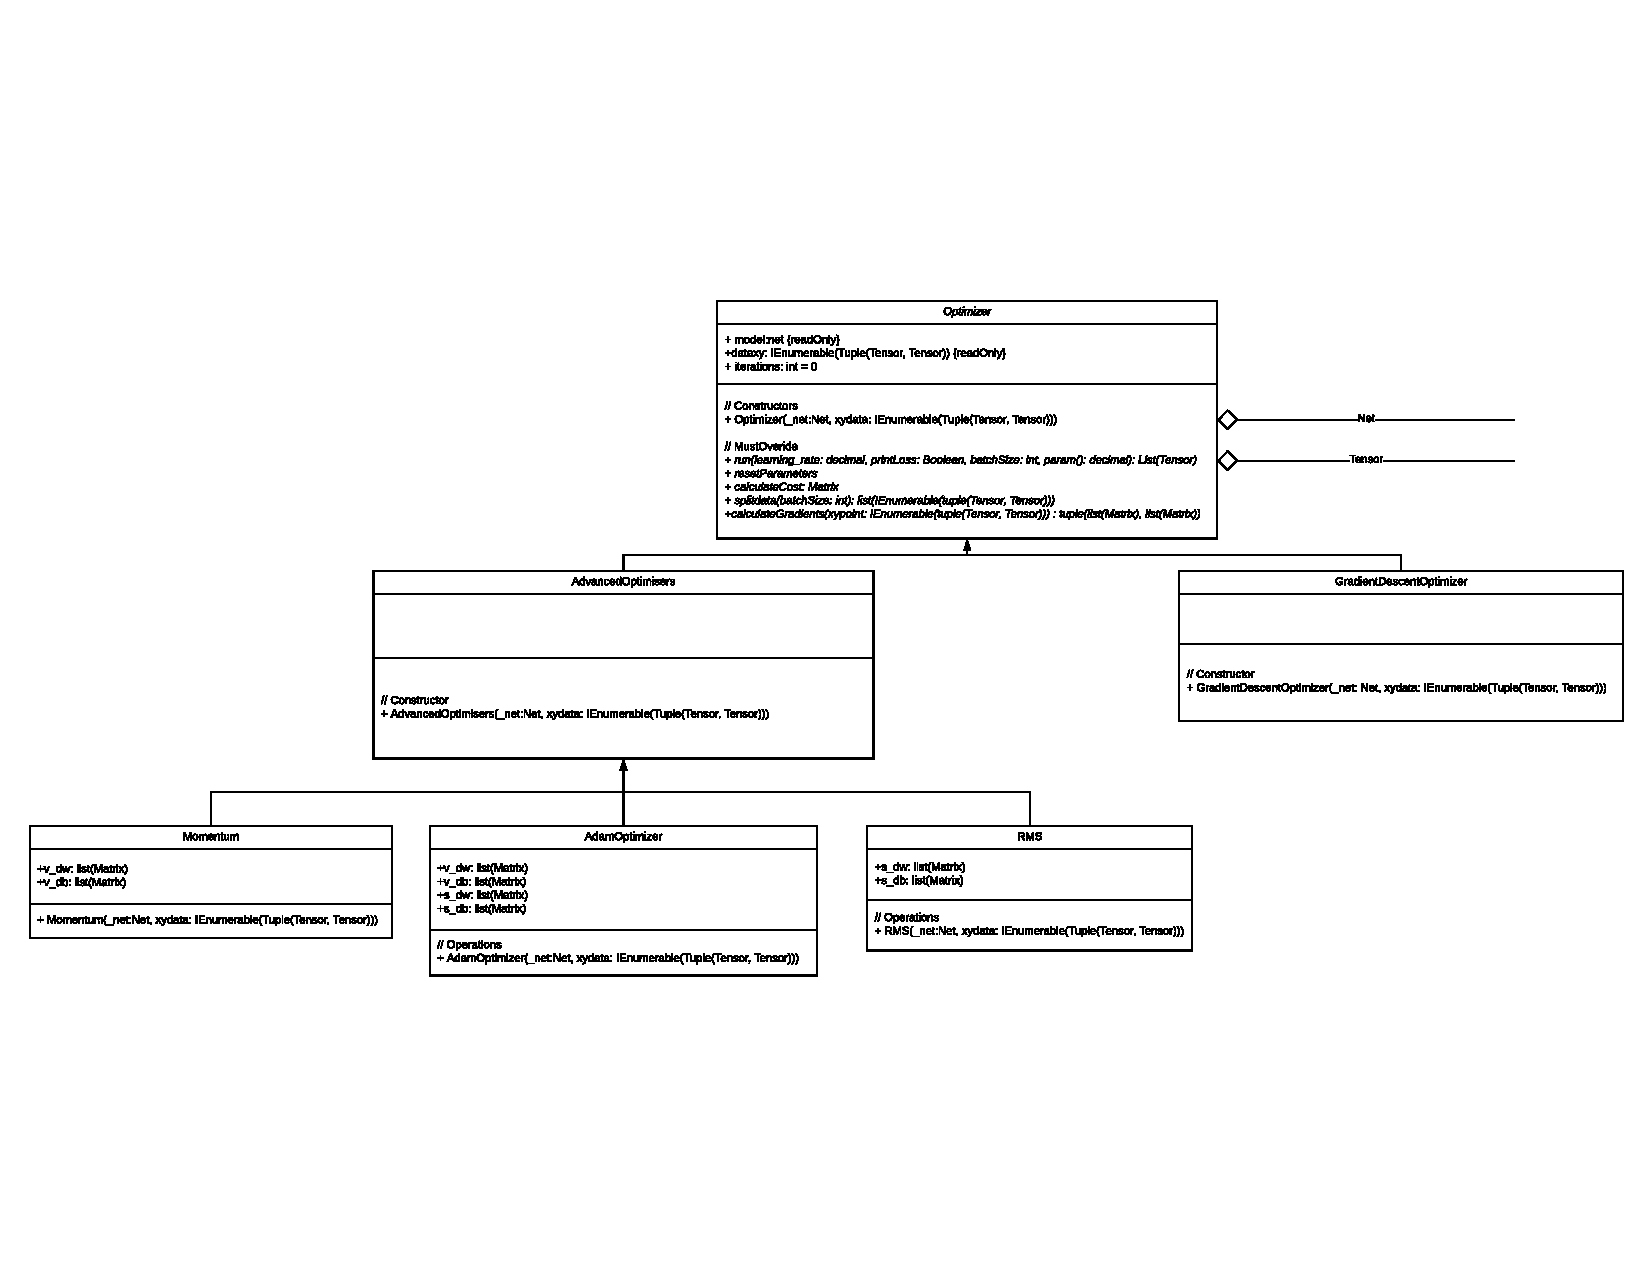
\includegraphics[width=18cm, height=18cm, angle=90]{Design/Overview/UMLCharts/NeuralDotUMLSeperated-Optimisers.pdf}
    \caption{Class Diagram for NeuralDot Library - Optimisers}
    \label{fig:Class Diagram for NeuralDot Library - Optimisers}
\end{figure}

\begin{figure}[H]
    \centering
    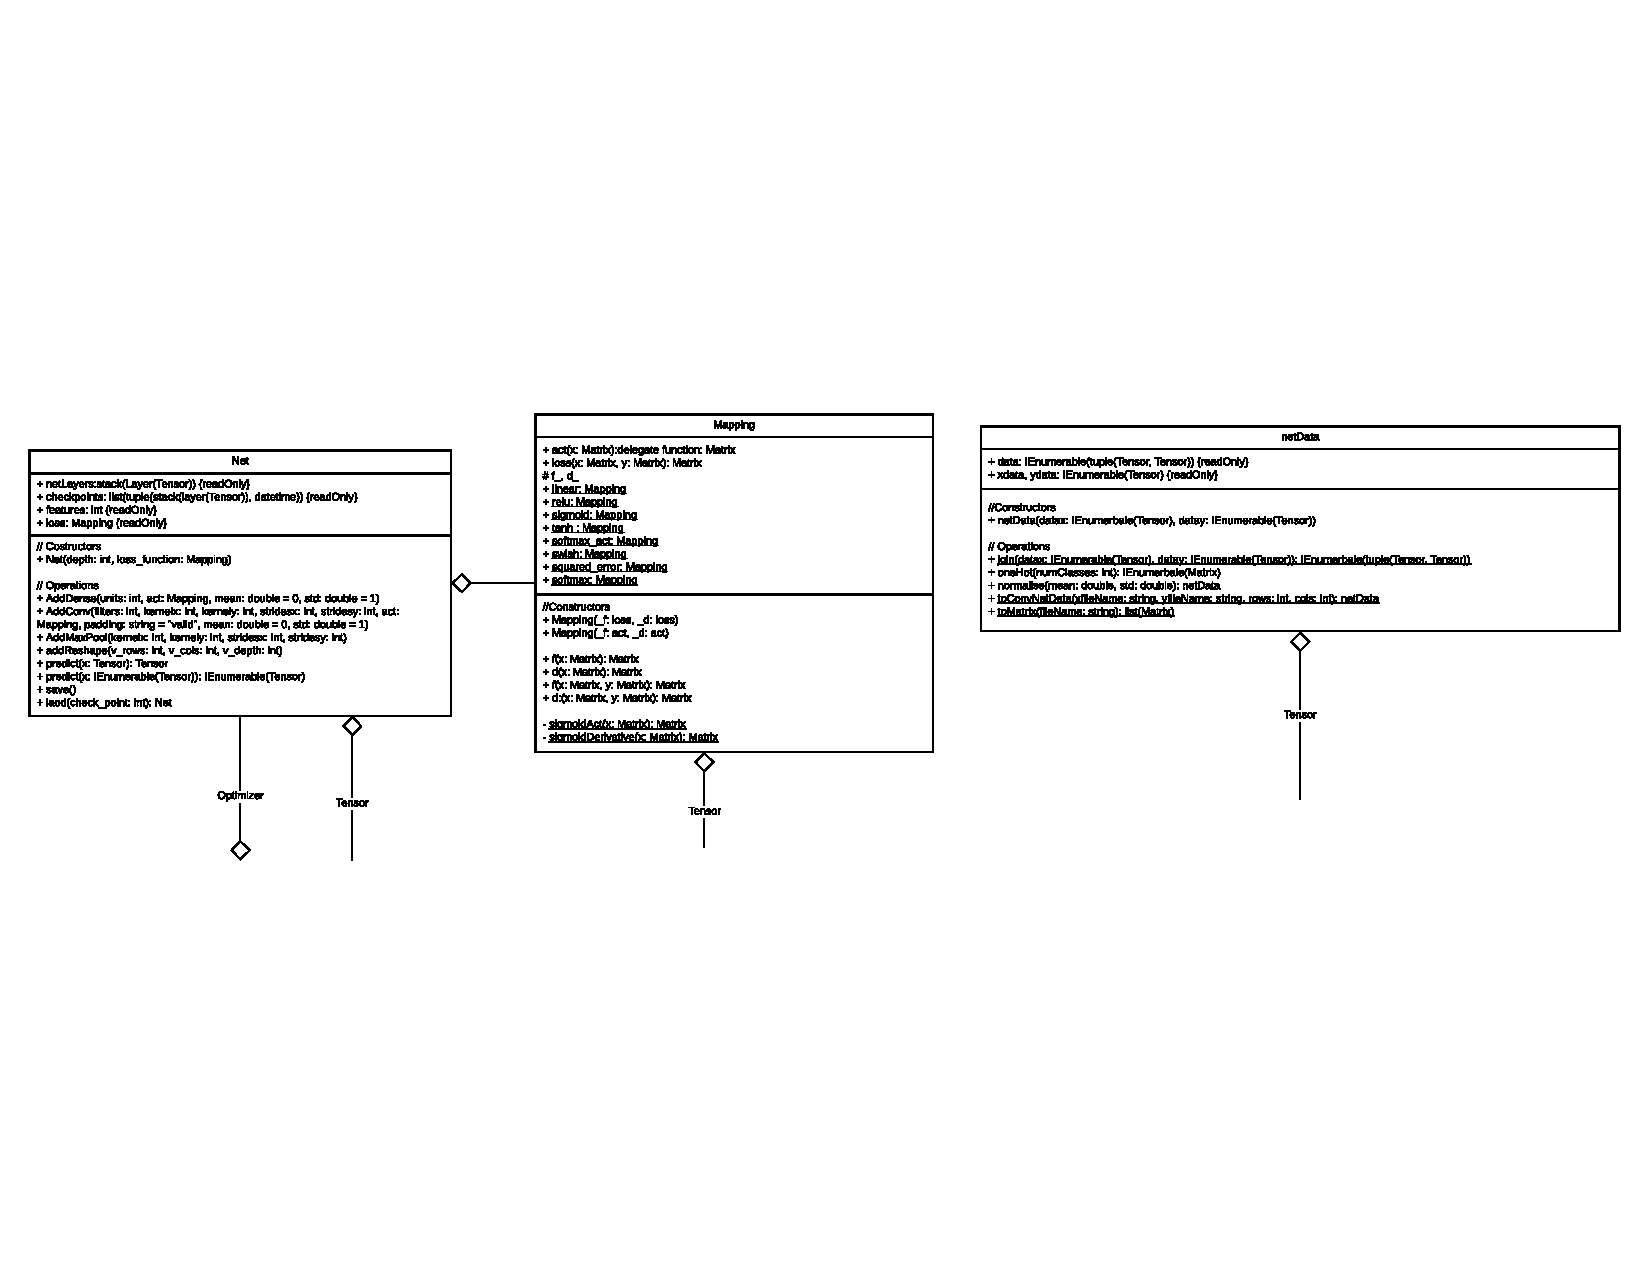
\includegraphics[width=18cm, height=18cm, angle=90]{Design/Overview/UMLCharts/NeuralDotUMLSeperated-Net.pdf}
    \caption{Class Diagram for NeuralDot Library - Net}
    \label{fig:Class Diagram for NeuralDot Library - Net}
\end{figure}

The figures above shows the UML for the NeuralDot library. The class \textbf{Tensor}, is a base class for the class \textbf{Matrix} and \textbf{Volume}, as both classes have functions in common. This base class is also necessary, as the \textbf{layers} class is a \textit{generic base class} of Tensor. Therefore, it is necessary to have \textbf{volume} and \textbf{matrix} \textit{inherit} from \textbf{Tensor}, as some layers will be of type \textbf{Volume}, and some of \textbf{Matrix}. The class \textbf{matrix} includes all the functions, iterators and subroutines that the user may use and the same applies for the \textbf{Volume} Class. In addition to the sub-routines, functions and iterators, I have also added \textit{shared operators} to both classes such as +, -, *, and /. These operators makes using matrices and volumes more accessible and intuitive for beginners making the library more user-friendly to work with.
\\ \\
The \textbf{Layer} class is a \textit{generic interface} of type \textbf{Tensor}. The classes \textbf{Dense}, \textbf{Conv}, \textbf{MaxPool} and \textbf{Reshape} all \textit{extend} from \textbf{Layer}, as they all have the same functions and are all layers. The class \textbf{Layer} includes all the main functionalities required by any specific layer such as updating the layer, retrieving the parameters and so on. Besides the class \textbf{Dense}, every other class that implements Layers, do not have any other functions besides the ones they override from the base class. The class \textbf{Dense}, which implements \textit{layer(Of Matrix)}, has 2 extra functions called gradient each which return the gradient for a particular back-prop iteration given the previous layers gradients, with the only difference being that one of them only works if it is the final layer in the net. These extra functions are there so that the advanced optimisation methods can then be used to train these dense nets, allowing the user to gain an intuition onto which optimisation method works best for which particular architecture or data. Furthermore, these extra functions also allow the user to view the gradients for a particular training iterations, which is something the user asked for in the interview process, therefore I have added these extra functions to the \textbf{Dense} class only as my main focus was on Dense nets.
\\ \\
Finally, the class \textbf{Net} adds functionality to the network enabling users to add layers to their net and choose the loss function being used as well as the activations at each layer. Another functionality, I added to the \textbf{Net} class is that I allowed the user to save models in a list, enabling the user to have many models. This is so that the user can then experiment with different architectures, optimisation techniques and loss functions and then compare the impact each has on the overall outcome on the Net. After saving these models, the user can then load the net back from the list, called checkpoints, and then re-use this loaded Net.

\section{User-Interface}
Due to my program being a library, I will not be having a proper user-interface. However I will be making my library as easy as possible to use as this is very clearly stated by my clients.
\\
The main method in which I will be interacting with my users are through exception handlers and comments I placed in my code. An important point to note about exception handlers however, is that there are 2 types. Ones that I purposefully placed in my code, and the other are because of the vb compiler finding error in my code or the users code. The second type of errors are something I will need to keep to a minimum, as the user will not know where the error is specifically. I will achieve this by thoroughly testing out my library and taking care of any overflow problems that could occur anywhere within my library. \\
On the other hand, exceptions written by myself, will provide the user with where they went wrong and details of how they can avoid it. These exceptions, will make the library more accessible for the user as they know exactly where they went wrong. \\
Finally, comments can also be used as a way to guide the users upon how certain algorithms work or what certain variables or parameters represent. This will allow the user to feel less restricted when using my library as they will know exactly what each function does at each stage.